\apendice{Especificación de diseño}

\section{Introducción}
En esta sección se habla sobre la fase de desarrollo software en la que definen la arquitectura, los procedimientos o los datos que se utilizan. Por lo tanto, se da solución

\section{Diseño de datos}

\subsection{Gramática}
Lo referente a la gramática me baso en el trabajo realizado en las anteriores versiones de Thoth\cite{thothv2} y obtengo la parte del núcleo. Según el diagrama obtenido de la documentación del proyecto, la clase Grammar esta compuesta de Production y esta a su vez de Symbol. Por medio de la interfaz TypeHandler se definen los tipos de gramáticas que existen\ref{fig:4.1}.

\begin{figure}[h]
\centering
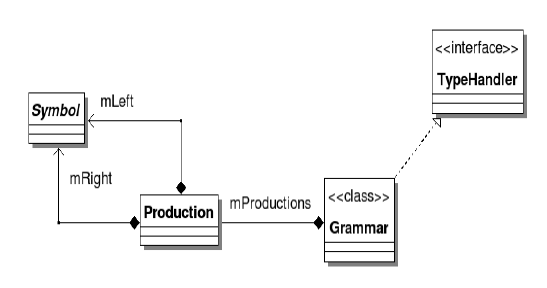
\includegraphics[width=0.50\textwidth]{diseno-gramatica}
\caption{Diagrama de clases del núcleo de la gramática\cite{thothv2}.}
\label{fig:4.1}
\end{figure}


\subsection{Símbolos}

Los símbolos son la unidad mínima con la que se trabajará en una gramática. Los símbolos en una gramática pueden ser terminales, no terminales. La clase NonTerminal estará formada por una cadena de terminales y la clase Terminal trabajará con un único carácter. También se definen los caracteres especiales como son epsilon, o el fin de cadena (TerminalEnd)\ref{fig:4.2}.

\begin{figure}[h]
\centering
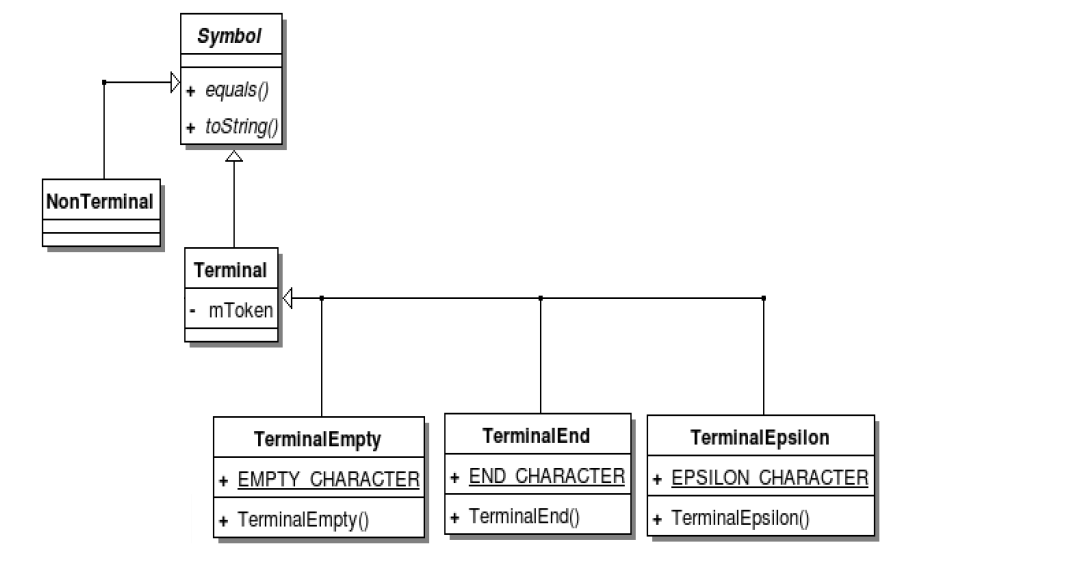
\includegraphics[width=0.60\textwidth]{diseno-simbolo}
\caption{Diagrama de clases de la estructura de Símbolo.}
\label{fig:4.2}
\end{figure}

La especificación de los caracteres que pertenecen a cada tipo viene impuesta por la sintaxis utilizada. Se decidió utilizar minúsculas, dígitos y los operadores básicos ($\ast,+,-,\cdot$) para los terminales. Para los no terminales se determinó que la primera letra debía ir en mayúscula y a ésta le podía seguir cualquier otro terminal o no terminal.

\subsection{Algoritmos de la gramática}

Por simplificación se decide juntar todos los algoritmos de limpieza de gramáticas en un mismo caso dentro del diagrama. Además su estructura es similar entre ellos.

En la figura\ref{fig:4.3} se aprecia como ~los algoritmos de limpieza tienen dos atributos principales, uno correspondiente a la gramática que se desea limpiar, definida como <<mOldGrammar>> y otro que representara la gramática resultante, <<mNewGrammar>>.

\begin{figure}[h]
\centering
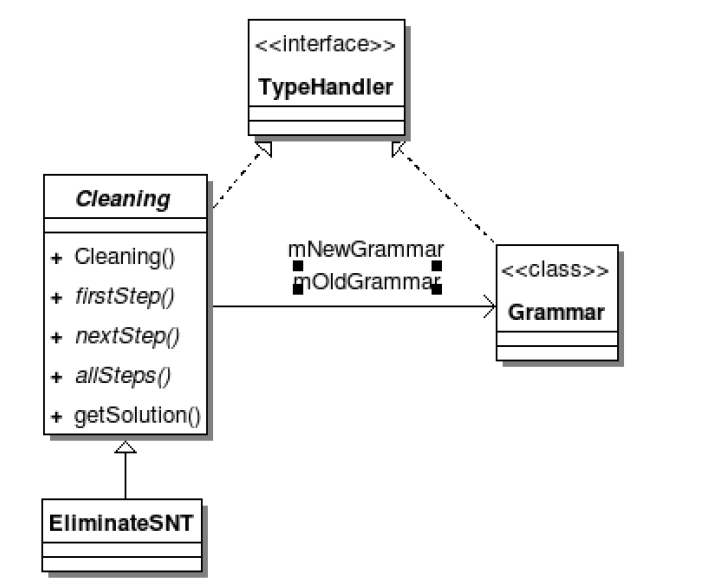
\includegraphics[width=0.40\textwidth]{diseno-algoritmos}
\caption{Diagrama de clases de los Algoritmos de la gramática\cite{thothv2}.}
\label{fig:4.3}
\end{figure}

\subsection{Parser de la gramática}

Aquí se define el diagrama mediante el cual el parser analiza la construcción de una gramática, en caso de estar correctamente construida nos crea la estructura interna propia, en caso de contener algún fallo nos muestra un error con el primer símbolo incorrecto encontrado.
A diferencia del parser de expresión regular aquí no se crea ningún árbol de
derivación, en su lugar se va analizando texto plano para ir creando la estructura interna propia.
Esta forma de construcción de gramáticas se ha realizado con el fin de no tener que construir una gramática cada nueva producción, solo se creará la gramática cuando queramos utilizarla (instanciación bajo demanda).

\begin{figure}[h]
\centering
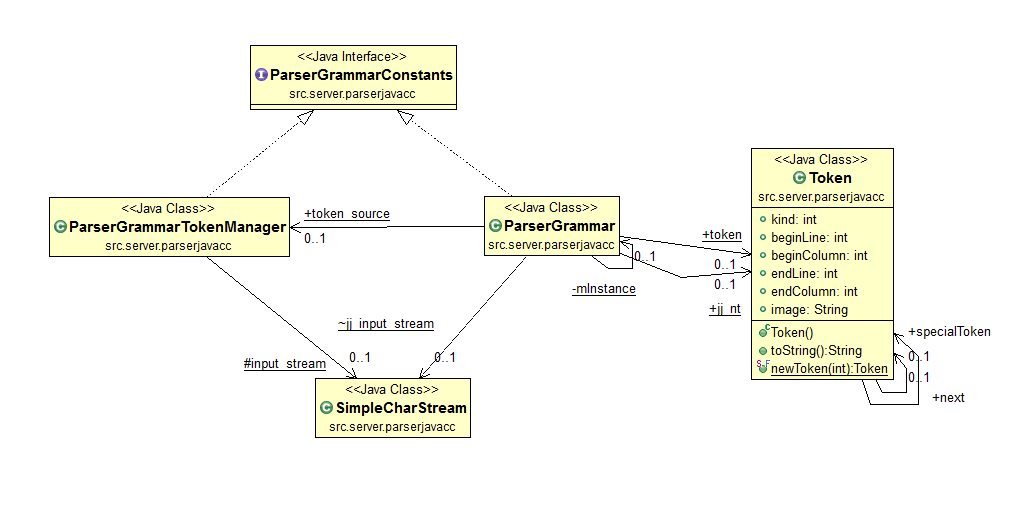
\includegraphics[width=1\textwidth]{diseno-parser}
\caption{Diagrama de clases del Parser de la gramática\cite{thothv2}.}
\label{fig:4.}
\end{figure}

\section{Diseño procedimental}

\section{Diseño arquitectónico}


